\subsection{Simplest ever XOR encryption}

I once saw a software where all debugging messages has been encrypted using XOR by value of 3.
In other words, two lowest bits of each character has been flipped.

``Hello, world'' would become ``Kfool/\#tlqog'':

\begin{lstlisting}[caption=Python,style=custompy]
#!/usr/bin/python

msg="Hello, world!"

print "".join(map(lambda x: chr(ord(x)^3), msg))
\end{lstlisting}

This is quite interesting encryption (or rather obfuscation), because it has two important properties:
1) single function for encryption/decryption, just apply it again;
2) resulting characters are also printable, so the whole string can be used in source code without escaping characters.

The second property exploits the fact that all printable characters organized in rows: 0x2x-0x7x, and when you 
flip two lowest bits, character \emph{moving} 1 or 3 characters left or right, but never \emph{moved} to another (maybe
non-printable) row:

\begin{figure}[H]
\centering
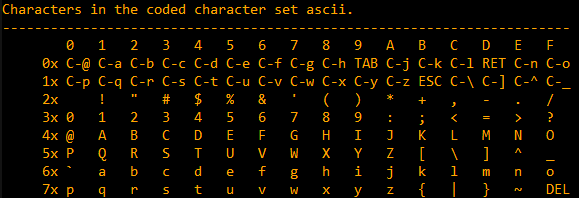
\includegraphics[width=0.8\textwidth]{ascii_clean.png}
\caption{7-bit \ac{ASCII} table in Emacs}
\end{figure}

\dots with a single exception of 0x7F character.

For example, let's \emph{encrypt} characters in A-Z range:

\begin{lstlisting}
#!/usr/bin/python

msg="@ABCDEFGHIJKLMNO"

print "".join(map(lambda x: chr(ord(x)^3), msg))
\end{lstlisting}

Result: \verb|CBA@GFEDKJIHONML|.

It's like ``@'' and ``C'' characters has been swapped, and so are ``B'' and ``a''.

Yet again, this is interesting example of exploiting XOR properties, rather than encryption:
the very same effect of \emph{preserving printableness} can be achieved while flipping any of lowest 4 bits,
in any combination.

